\chapter{Effects of input scaling and loss balance}
In this chapter, we analyze and discuss the impact of input scaling and balancing the loss terms on the performance four MRI-based anisotropic PINN model. 
\section{Input Scaling}
As discussed in \ref{scaling}, input scaling is an important step in training neural networks, ensuring that input features contribute equally during training.
Figure \ref{fig:loss_aniso_no_scaling} shows the convergence of the training loss components of an anisotropic and heterogeneous MRI-based model. We see most (apart from $\mathcal{L}_{IC}$) loss components plateauing at higher values compared to \ref{fig:loss_aniso}. The final values of the loss components are summarized in Table\ref{tab:scaling}.
\begin{figure}[H]
  \centering
  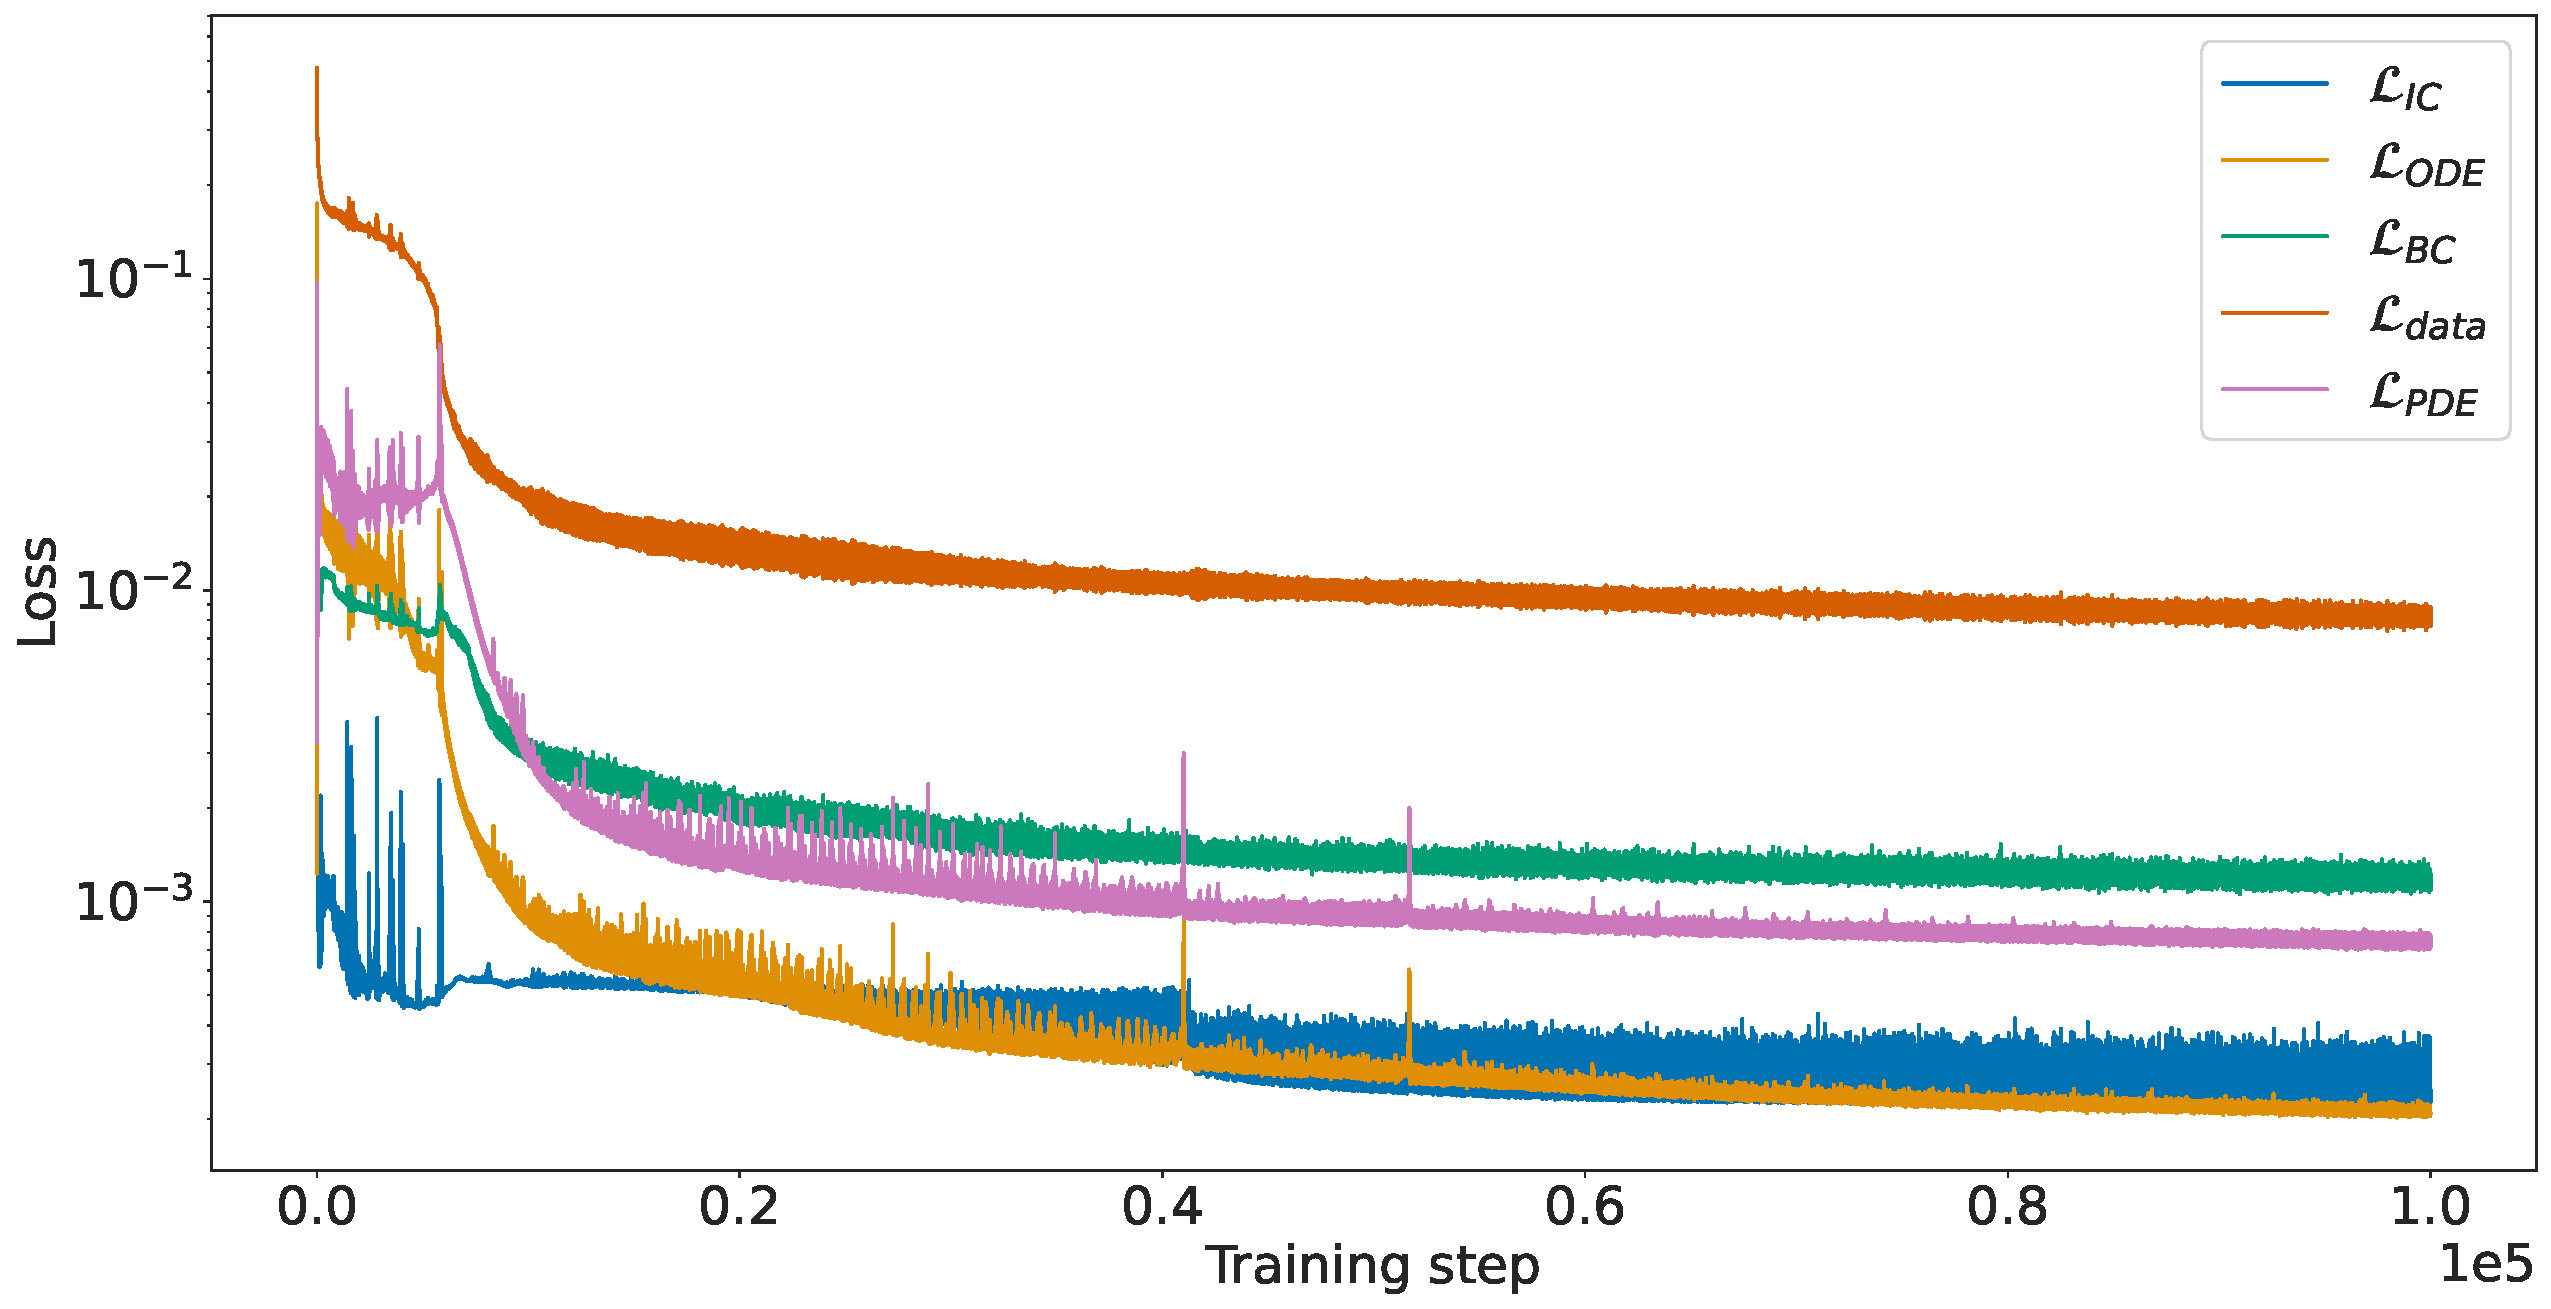
\includegraphics[width=\linewidth]{Figs/Anisotropic/loss_all_noscaling.pdf}
  \caption{Anisotropic and heterogeneous MRI-based model training loss convergence during training on a logarithmic scale. The plot shows the evolution of different components of the total loss when the model is trained without input scaling.}
  \label{fig:loss_aniso_no_scaling}
\end{figure}
\begin{table}[h]
  \centering
  \begin{tabular}{|c|c|c|}
    \hline
    component & With scaling & Without scaling \\ \hline
    $\mathcal{L}_{PDE}$  & $3.7\times 10^{-4}$  & $7.1\times 10^{-4}$  \\ \hline
    $\mathcal{L}_{ODE}$  & $7.0\times 10^{-5}$   & $2.1\times 10^{-4}$  \\ \hline
    $\mathcal{L}_{BC}$  & $1.6\times 10^{-4}$   & $1.2\times 10^{-3}$  \\ \hline
    $\mathcal{L}_{IC}$  & $2.5\times 10^{-4}$  & $2.2\times 10^{-4}$  \\ \hline
    $\mathcal{L}_{data}$ & $3.4\times 10^{-3}$  & $7.7\times 10^{-3}$  \\ \hline
    
  \end{tabular}
  \caption{Final training losses with and without input scaling}
  \label{tab:scaling}
\end{table}
Figure \ref{fig:RL1_anisotropic_no_scaling} shows the relative $L^1$ error when training without scaling the inputs. The plot shows higher errors in general, compared to scaling (Figure \ref{fig:RL1_anisotropic}) as well as an increase of the error for higher conductivities. Considering the difference in magnitudes of the inputs (the largest conductivity values being of two orders of magnitude smaller than the largest spatio-temporal coordinate values), this suggests that the conductivity inputs become less significant during training due to the absence of input scaling.
\begin{figure}[H]
  \centering
  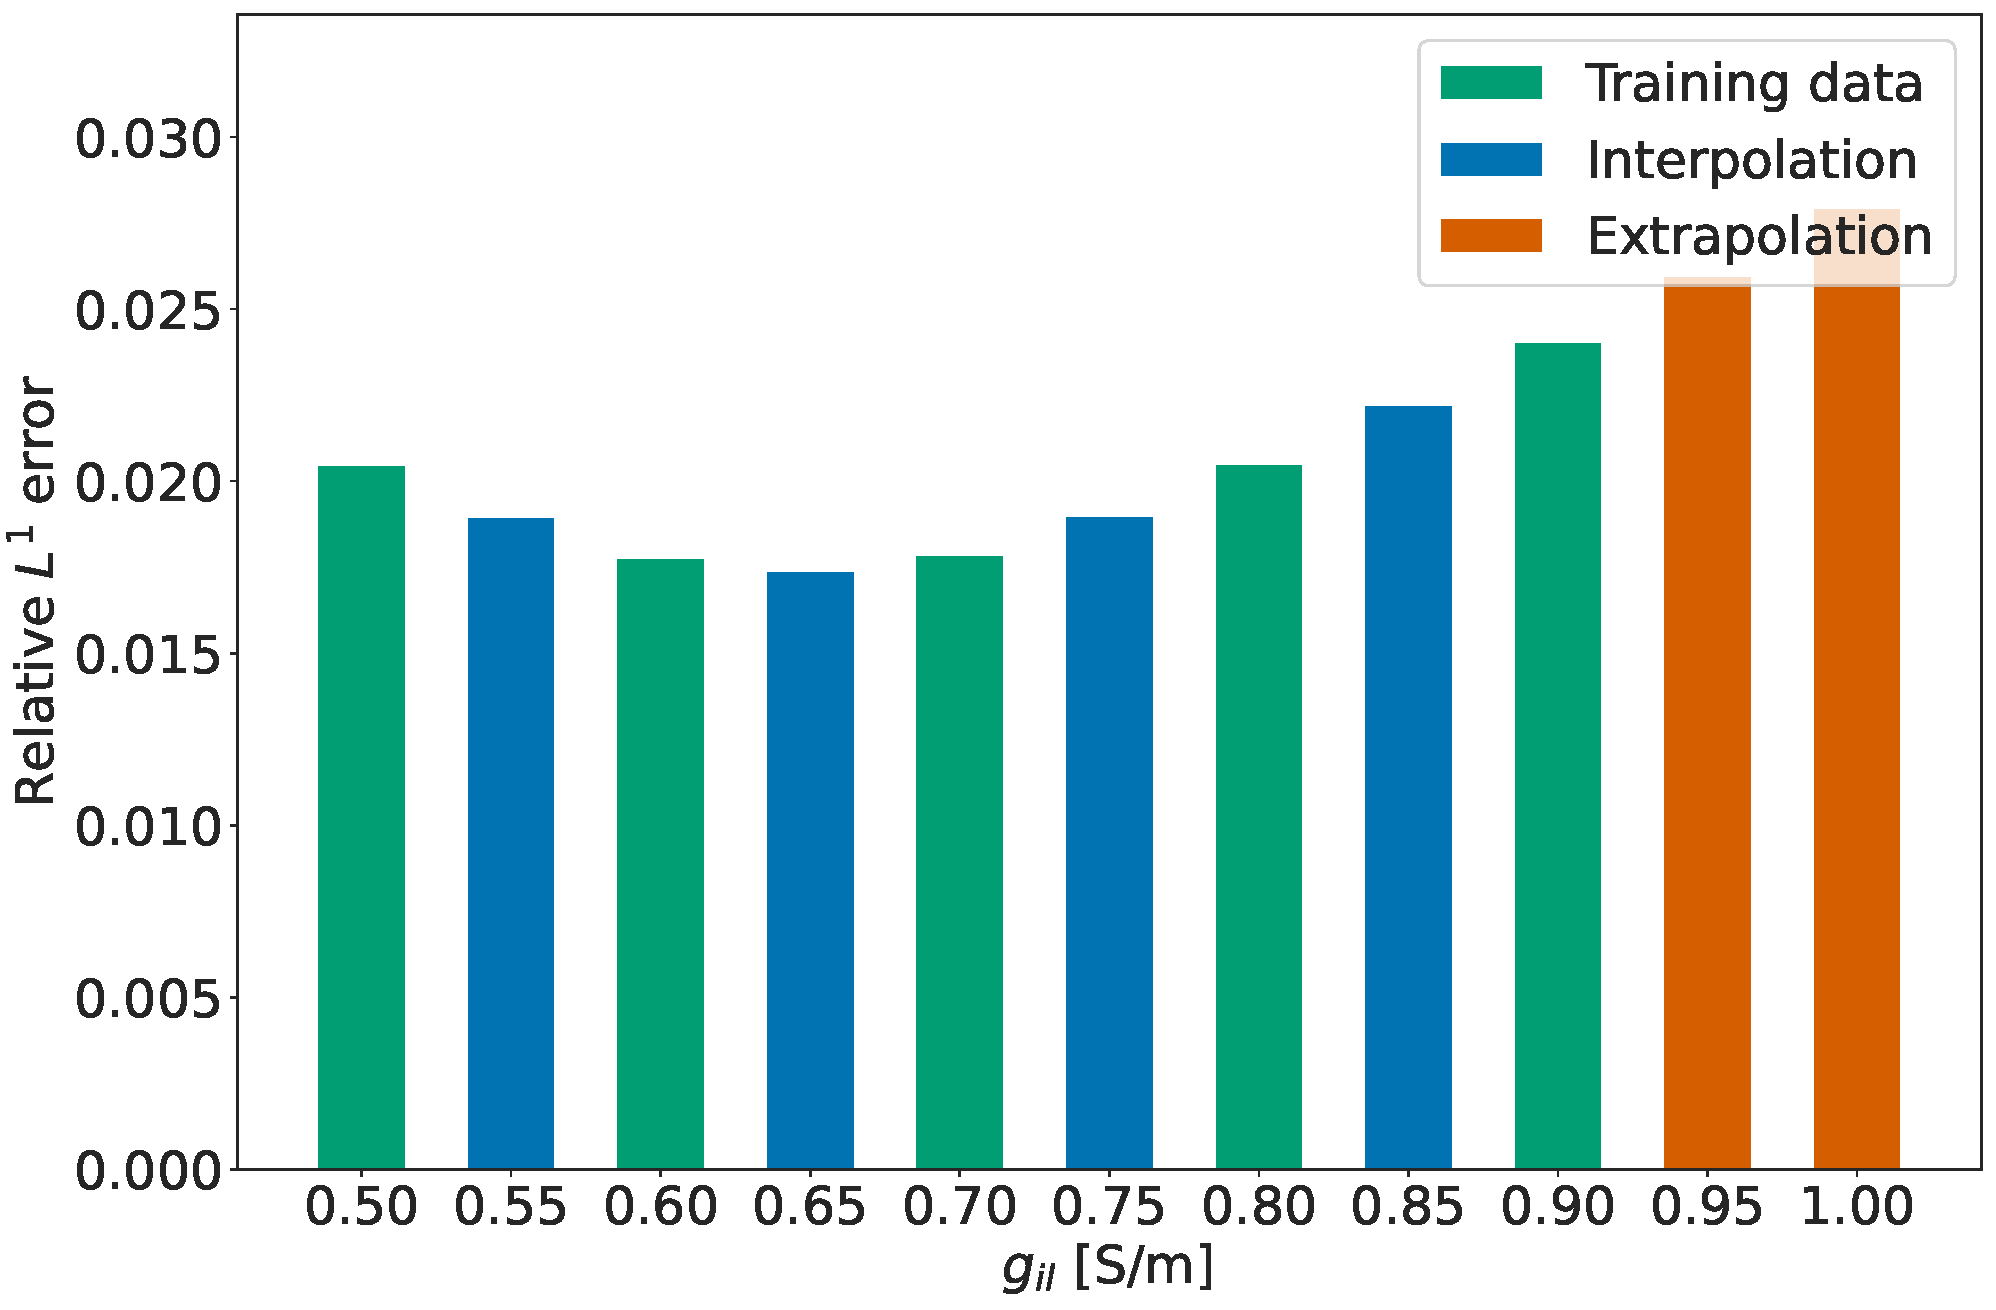
\includegraphics[width=0.8\linewidth]{Figs/Anisotropic/L1_error_bar_plot_no_scaling.pdf}
  \caption{Relative $L^1$ error computed from MRI-based model with anisotropic and heterogeneous conductivities trained without input scaling.}
  \label{fig:RL1_anisotropic_no_scaling}
\end{figure}


\section{Loss balance}
As discussed in \ref{loss_balance}, balancing the contribution of each loss component during training is cricial when the different components have different magnitudes. By balancing these losses, we ensure that no single component dominates the optimization process.

Figure \ref{fig:loss_aniso_no_relobralo} shows the convergence of the training loss components of an anisotropic and heterogeneous MRI-based model. We see all loss components converging faster, but plateauing at higher values compared to \ref{fig:loss_aniso}. The final values of the loss components are summarized in Table\ref{tab:no_relobralo}.
\begin{figure}[H]
  \centering
  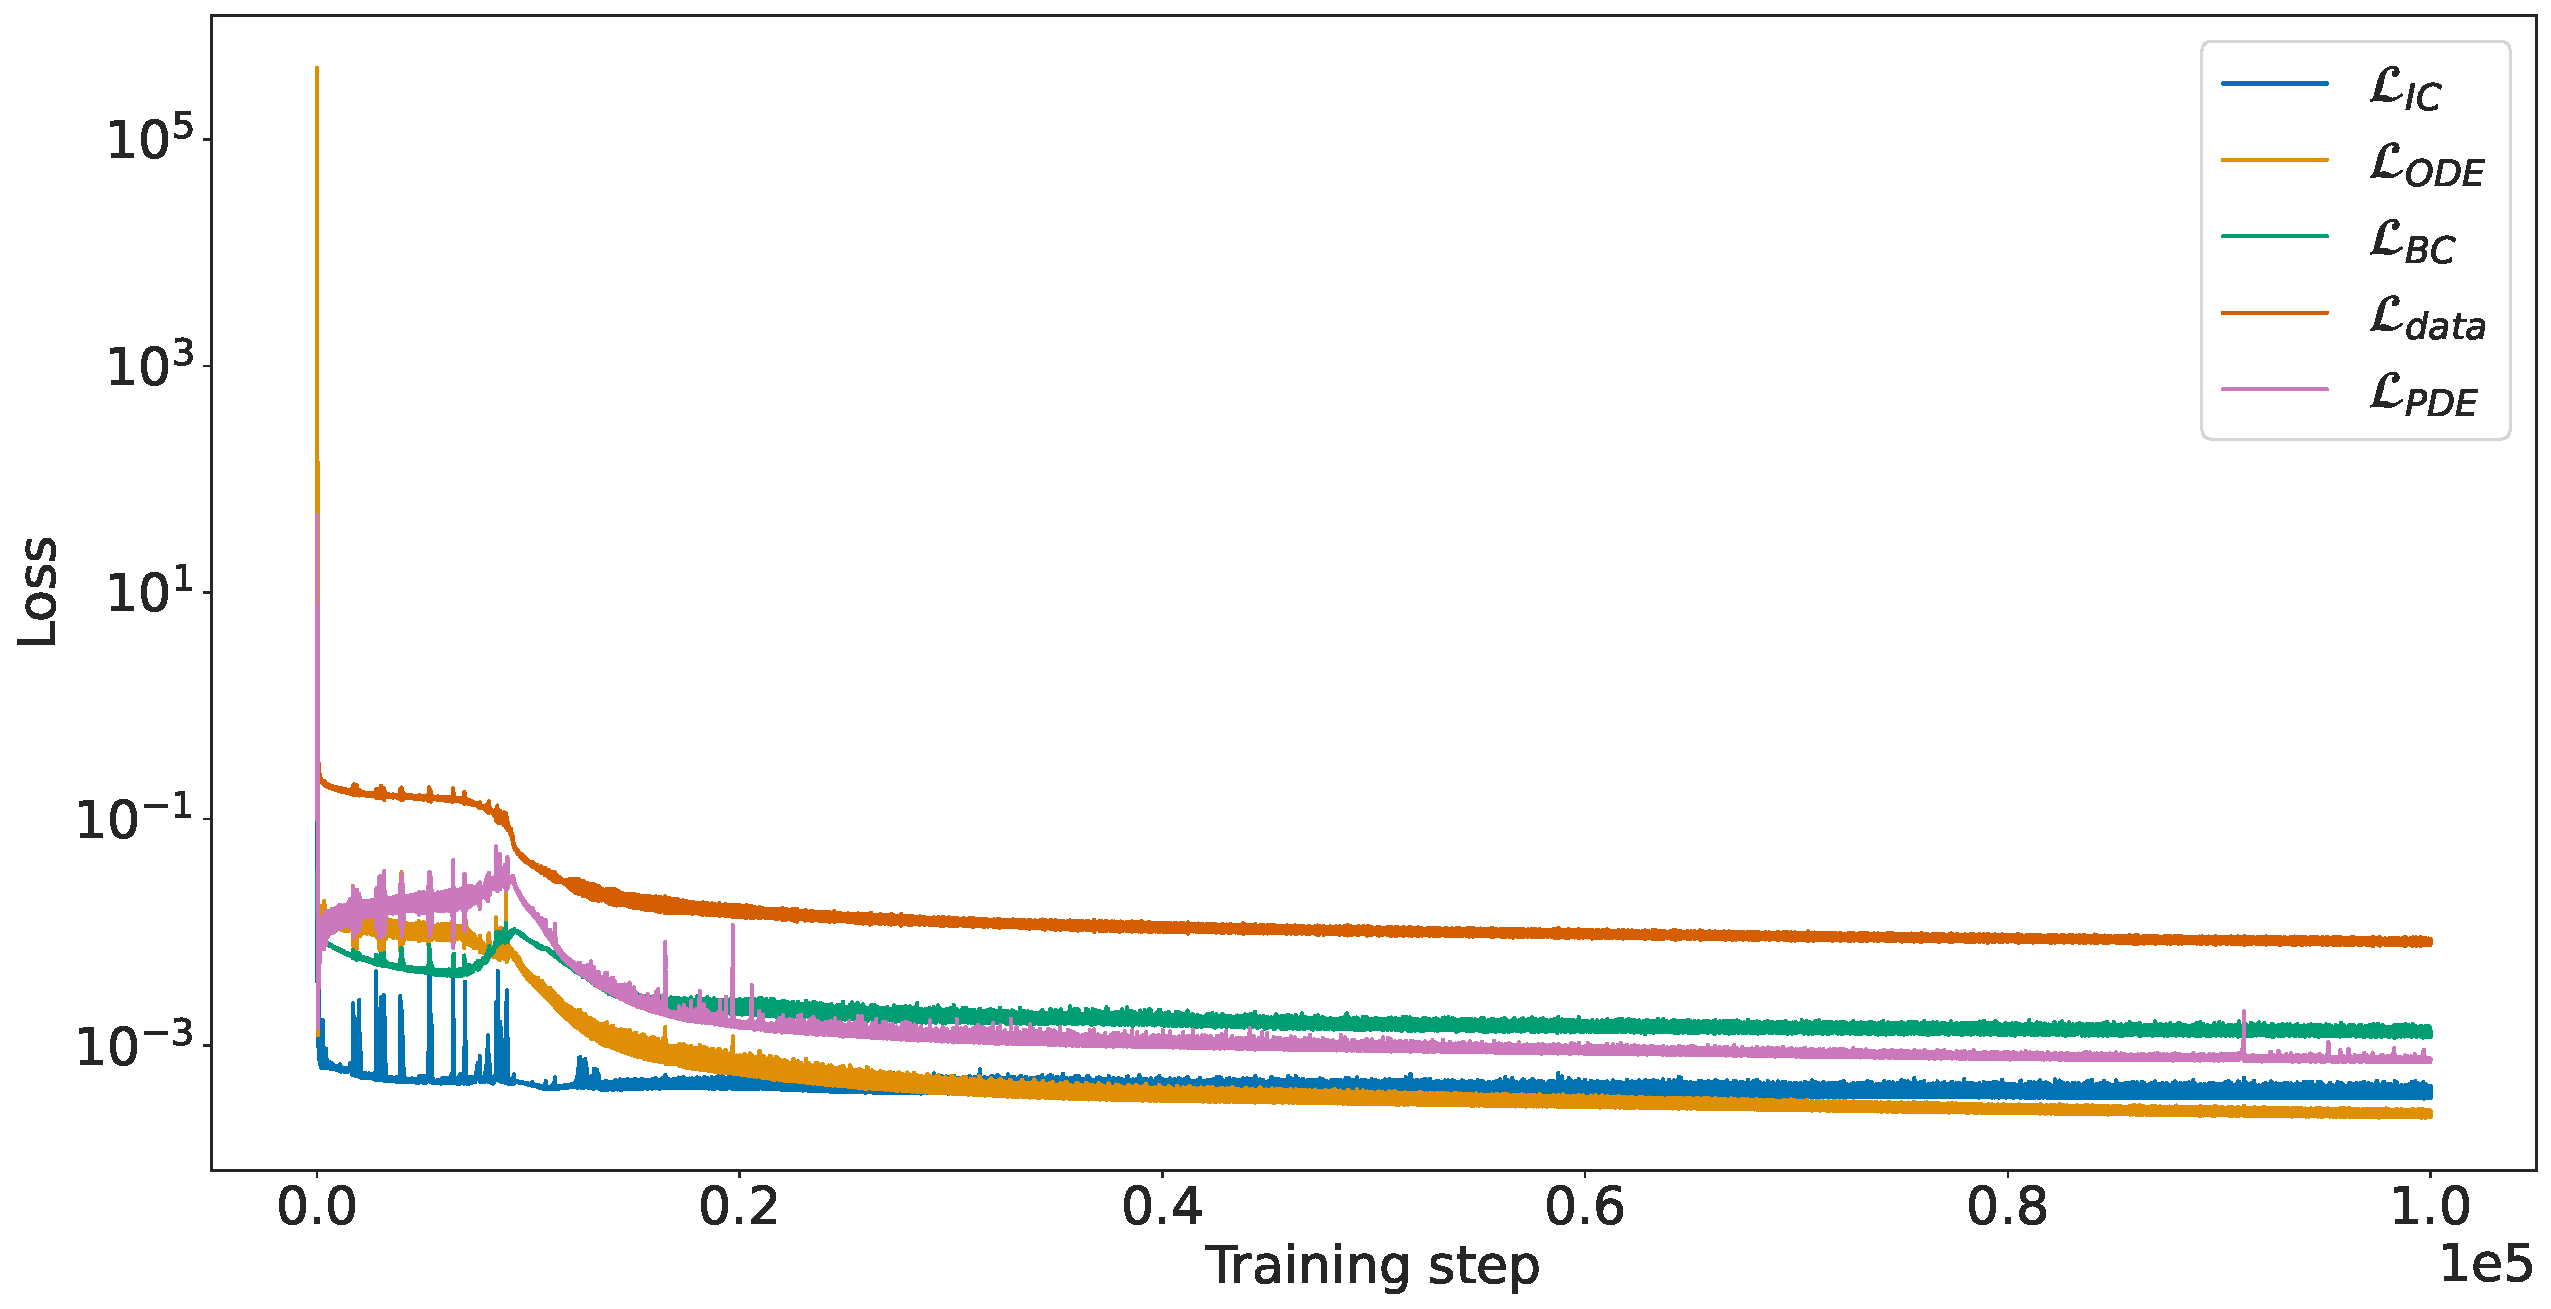
\includegraphics[width=\linewidth]{Figs/Anisotropic/loss_aniso_no_relobralo.pdf}
  \caption{Anisotropic and heterogeneous MRI-based model training loss convergence during training on a logarithmic scale. The plot shows the evolution of different components of the total loss when the model is trained with all loss weights set to one  ($\lambda_i=1$).}
  \label{fig:loss_aniso_no_relobralo}
\end{figure}

\begin{table}[h]
  \centering
  \begin{tabular}{|c|c|c|}
    \hline
    component & ReLoBRaLo & Without ReLoBRaLo  \\ \hline
    $\mathcal{L}_{PDE}$  & $3.7\times 10^{-4}$  & $7.6\times 10^{-4}$   \\ \hline
    $\mathcal{L}_{ODE}$  & $7.0\times 10^{-5}$   & $2.7\times 10^{-4}$   \\ \hline
    $\mathcal{L}_{BC}$  & $1.6\times 10^{-4}$   & $1.3\times 10^{-3}$  \\ \hline
    $\mathcal{L}_{IC}$  & $2.5\times 10^{-4}$  & $3.5\times 10^{-4}$ \\ \hline
    $\mathcal{L}_{data}$ & $3.4\times 10^{-3}$  & $8.1\times 10^{-3}$  \\ \hline
    
  \end{tabular}
  \caption{Final training losses with and without loss term balancing (ReLoBRaLo)}
  \label{tab:no_relobralo}
\end{table}

Figure \ref{fig:RL1_anisotropic_no_relobralo} illustrates the relative $L^1$ errors for the model trained without balancing the loss terms. The errors are less consistent at the lower en of $g_il$ values, indication that the lack of loss term balancing results in less reliable performance.
\begin{figure}[H]
  \centering
  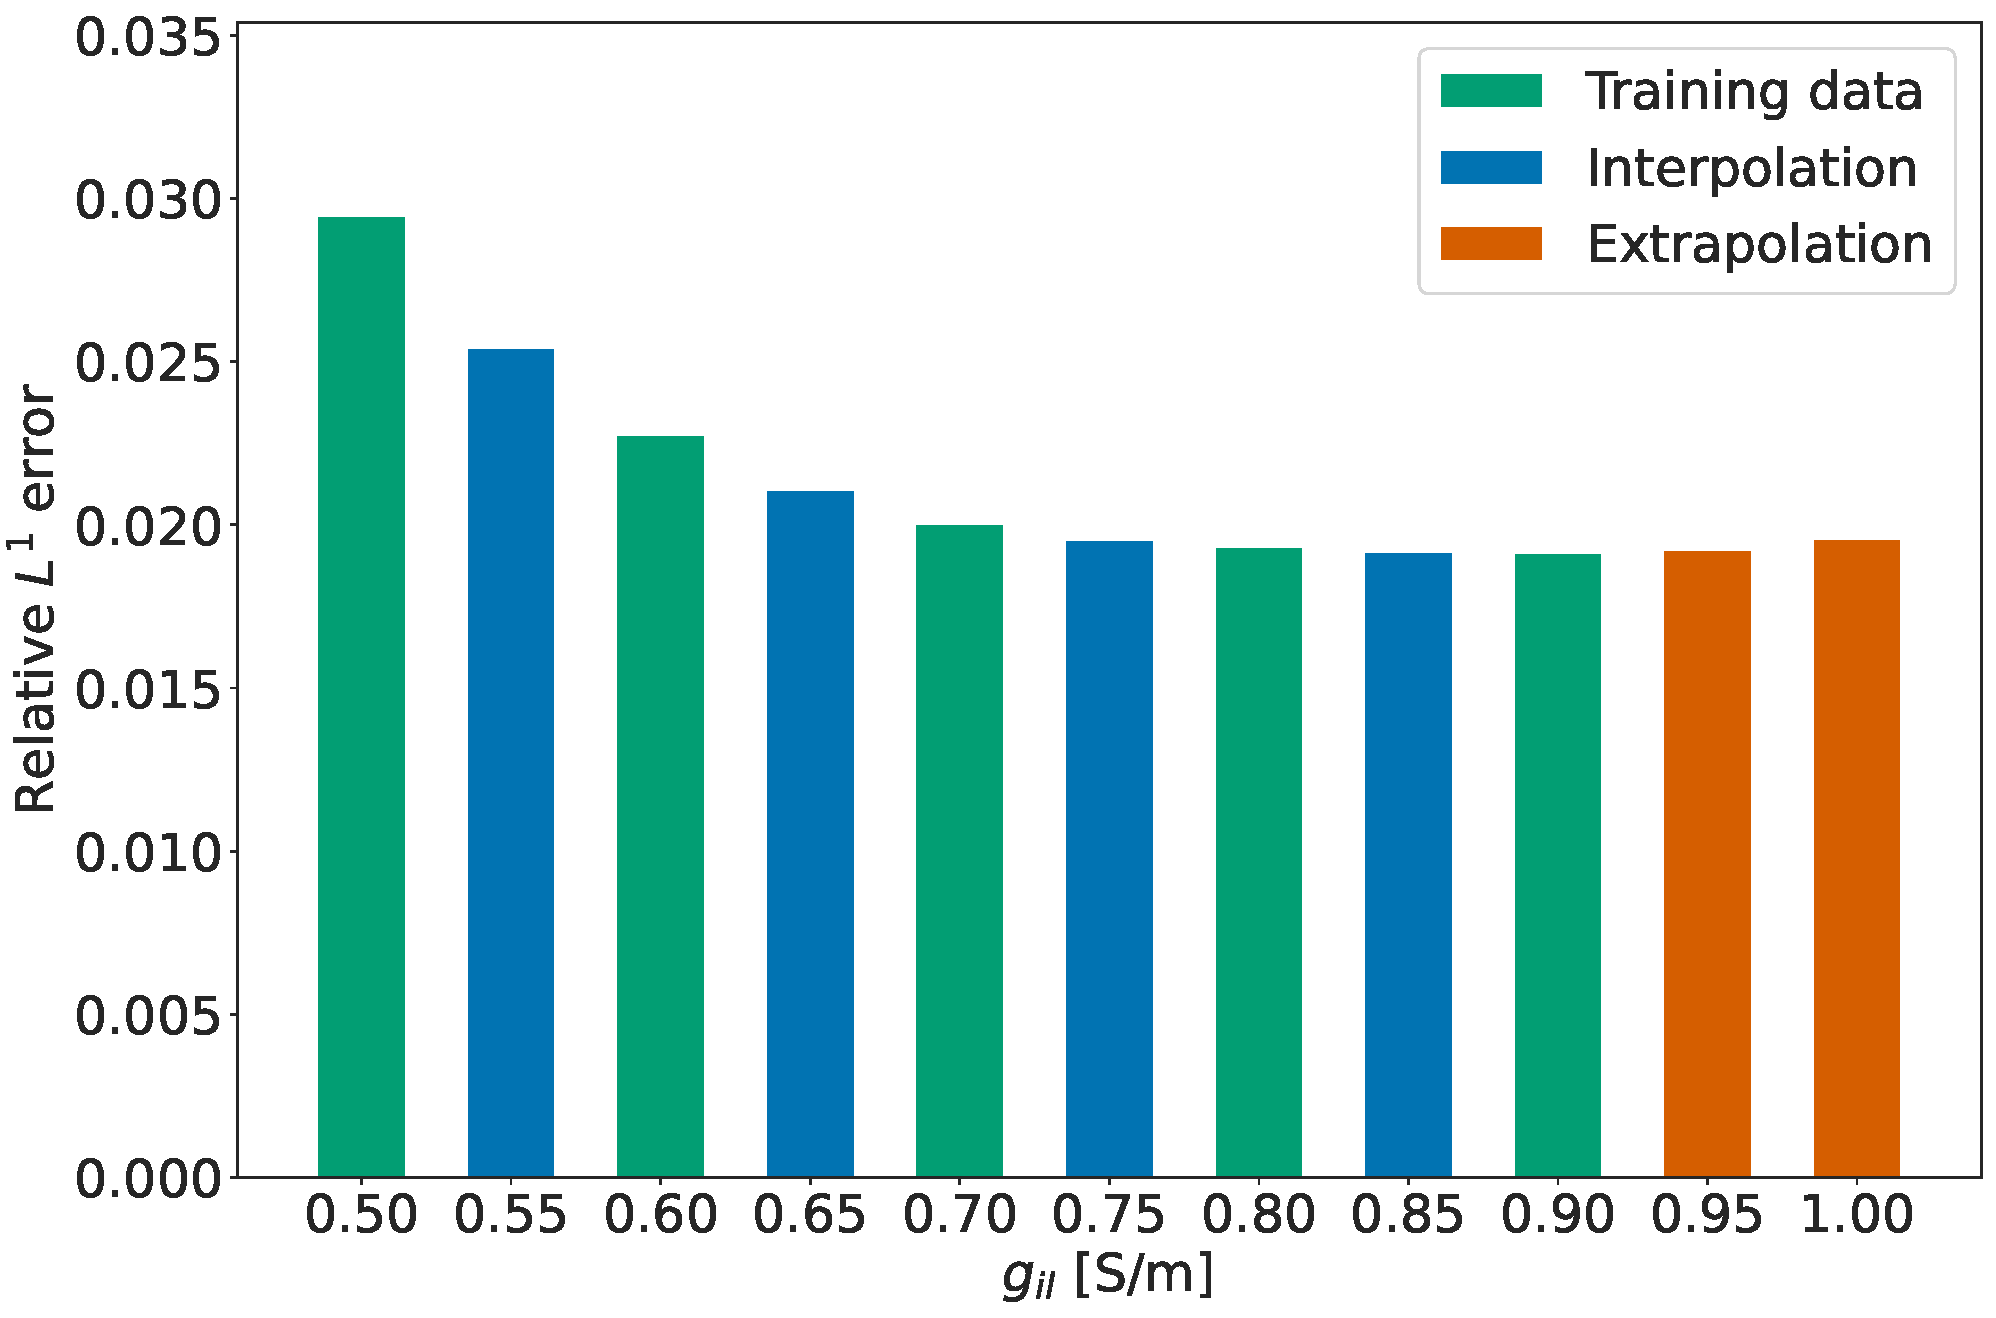
\includegraphics[width=0.8\linewidth]{Figs/Anisotropic/L1_error_bar_plot_no_relobralo.pdf}
  \caption{Relative $L^1$ error computed from MRI-based model with anisotropic and heterogeneous conductivities trained with $\lambda_i=1$.}
  \label{fig:RL1_anisotropic_no_relobralo}
\end{figure}


\chapter{Computing in Cardiology Conference Abstract Submission}
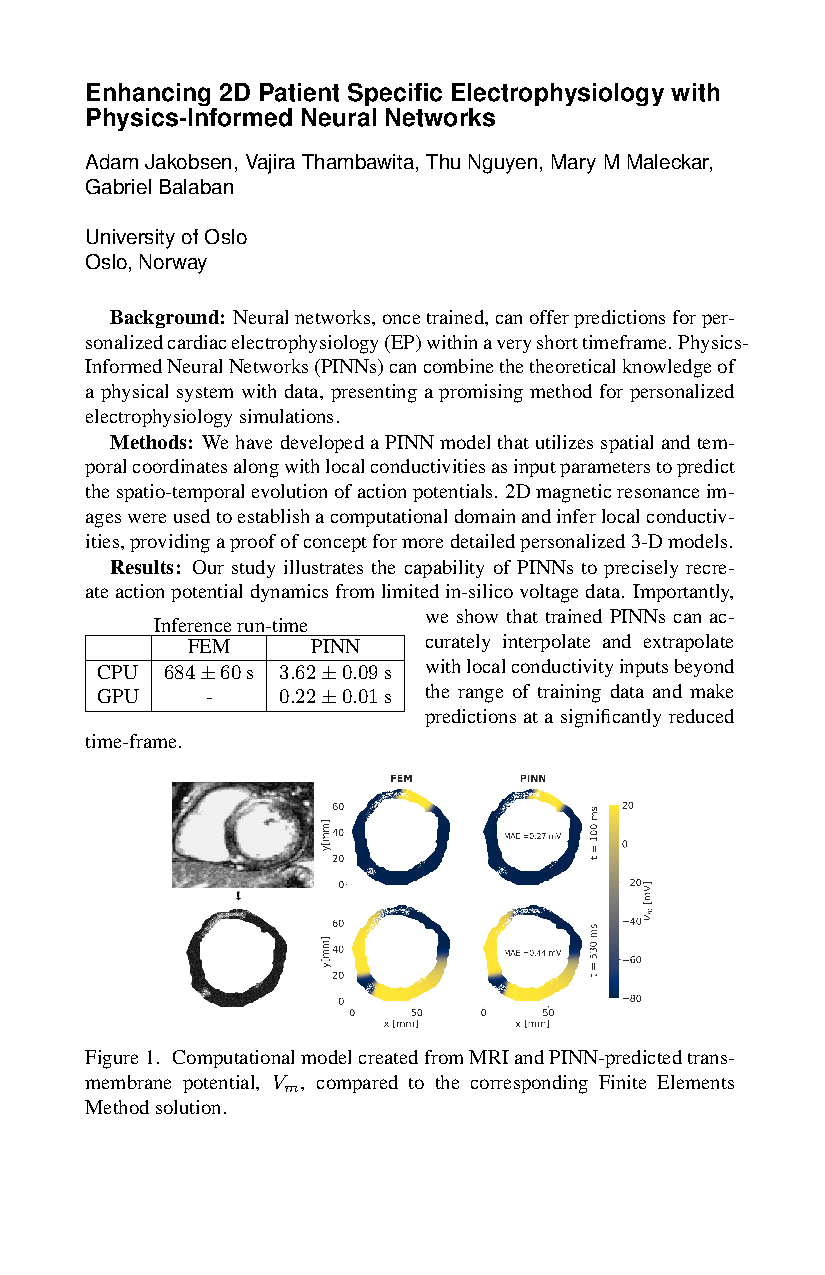
\includepdf[pages=-]{Cinc24.pdf}
